% !TEX program = XeLaTeX
% !TEX encoding = UTF-8

\documentclass[a4paper]{article}

\usepackage[UTF8]{ctex}
\usepackage{graphicx}
\usepackage{soul, color, xcolor}
\usepackage[margin=1.25in]{geometry}
\usepackage{amsfonts, amsmath, amsthm, bm, amssymb}
\usepackage{float}
\usepackage{diagbox}
\usepackage{multirow}
\usepackage{hyperref}
\usepackage{listings}
\usepackage{tcolorbox}

% Times Math Font + Google Noto Font
\usepackage{txfonts}
\usepackage{fontspec}
\setmainfont{Noto Serif Regular}[BoldFont = Noto Serif Bold, ItalicFont = Noto Serif Italic, BoldItalicFont = Noto Serif BoldItalic]
\setsansfont{Noto Sans Regular}[BoldFont = Noto Sans Bold, ItalicFont = Noto Sans Italic, BoldItalicFont = Noto Sans BoldItalic]
\setmonofont{Noto Sans Mono Regular}[BoldFont = Noto Sans Mono Bold]
\setCJKmainfont{Noto Serif CJK SC Regular}[BoldFont = Noto Serif CJK SC Bold, ItalicFont = Noto Serif CJK SC Italic, BoldItalicFont = Noto Serif CJK SC BoldItalic]
\setCJKsansfont{Noto Sans CJK SC Regular}[BoldFont = Noto Sans CJK SC Bold, ItalicFont = Noto Sans CJK SC Italic, BoldItalicFont = Noto Sans CJK SC BoldItalic]
\setCJKmonofont{Noto Sans Mono CJK SC Regular}[BoldFont = Noto Sans Mono CJK SC Bold]

\lstset{basicstyle=\small\ttfamily}

\setlength{\parindent}{0pt}

\numberwithin{equation}{section}

\theoremstyle{definition}
\newtheorem*{solution}{Solution}
\newtheorem*{prove}{Proof}

\def \transposed {\mathsf{T}}
\def \hermitian {\mathsf{H}}
\def \Real {\mathbb{R}}
\def \betaBold {\bm{\beta}}
\def \lambdaBold {\bm{\lambda}}
\def \LambdaBold {\bm{\Lambda}}
\def \MuBold {\bm{\Mu}}
\def \muBold {\bm{\mu}}
\def \Sw {\mathbf{S}_{\operatorname{w}}}
\def \Sb {\mathbf{S}_{\operatorname{b}}}
\def \St {\mathbf{S}_{\operatorname{t}}}
\def \A {\mathbf{A}}
\def \B {\mathbf{B}}
\def \C {\mathbf{C}}
\def \O {\mathbf{O}}
\def \P {\mathbf{P}}
\def \Q {\mathbf{Q}}
\def \I {\mathbf{I}}
\def \S {\mathbf{S}}
\def \M {\mathbf{M}}
\def \W {\mathbf{W}}
\def \X {\mathbf{X}}
\def \u {\bm{u}}
\def \v {\bm{v}}
\def \w {\bm{w}}
\def \wh {\hat{\bm{w}}}
\def \ws {\bm{w}^\star}
\def \y {\bm{y}}
\def \x {\bm{x}}
\def \xh {\hat{\bm{x}}}

\def \MI {\operatorname{MI}}
\def \Ent {\operatorname{Ent}}

% \let\oldnorm\norm
% \let\norm\undefined
\newcommand\abs[1]{\left| #1 \right|}
\newcommand\norm[1]{\left\| #1 \right\|}
\newcommand\inner[2]{\left\langle #1, #2 \right\rangle}
\newcommand\sbr[1]{\left( #1 \right)}
\newcommand\mbr[1]{\left[ #1 \right]}
\newcommand\lbr[1]{\left\{#1 \right\}}
\newcommand\tr[1]{\operatorname{tr}\sbr{#1}}
\newcommand\rank[1]{\operatorname{rank}\sbr{#1}}
\newcommand\indicator[1]{\mathbb{I}\sbr{#1}}

\begin{document}

\title{机器学习导论 习题二}
% \author{学号, 姓名, \href{mailto:邮箱}{邮箱}}
\author{参考答案}
\maketitle

% \section*{作业注意事项}

% \begin{tcolorbox}
%     \begin{enumerate}
%         \item[1.] 作业所需的LaTeX及Python环境配置要求请参考: \href{https://www.lamda.nju.edu.cn/ML2024Spring/supplementary/environment.pdf}{[Link]};
%         \item[2.] 请在LaTeX模板中第一页填写个人的学号、姓名、邮箱;
%         \item[3.] 本次作业需提交的文件与对应的命名方式为:
%               \begin{enumerate}
%                   \item [(a)] 作答后的LaTeX代码 --- \texttt{HW2.tex};
%                   \item [(b)] 由(a)编译得到的PDF文件 --- \texttt{HW2.pdf};
%                   \item [(c)] 编程题代码 --- \texttt{main.py};
%               \end{enumerate}
%               请将以上文件{\color{red}\textbf{打包为 ``\texttt{学号\hspace{0em}\_\hspace{0em}姓名.zip}''}}~(例如 ``\texttt{221300001\_\hspace{0em}张三.zip}'') 后提交;
%         \item[3.] 若多次提交作业, 则在命名 ``\texttt{.zip}'' 文件时加上版本号, 例如 ``\texttt{221300001\_\hspace{0em}张三\hspace{0em}\_v1.zip}'' (批改时以版本号最高, 提交时间最新的文件为准);
%         \item[4.] 本次作业提交截止时间为~{\color{red}\textbf{{4}月{16}日{23:59:59}}}. 未按照要求提交作业, 提交作业格式不正确, {\color{red}\textbf{作业命名不规范}}, 将会被扣除部分作业分数; 除特殊原因 (如因病缓交, 需出示医院假条) 逾期未交作业, 本次作业记 0 分; {\color{red}\textbf{如发现抄袭, 抄袭和被抄袭双方成绩全部取消}};
%         \item[5.] 学习过程中, 允许参考 ChatGPT 等生成式语言模型的生成结果, 但必须在可信的信息源处核实信息的真实性; {\color{red}\textbf{不允许直接使用模型的生成结果作为作业的回答内容}}, 否则将视为作业非本人完成并取消成绩;
%         \item[6.] 证明题请给出关键证明步骤, 计算题请列出算式及中间结果, 否则不予计分; 撰写数学表达式请遵循符号约定.
%         \item[7.] 本次作业提交地址为 \href{https://box.nju.edu.cn/u/d/a84222be492048779a27/}{[Link]}, 请大家预留时间提前上交, 以防在临近截止日期时, 因网络等原因无法按时提交作业.
%     \end{enumerate}
% \end{tcolorbox}

% \newpage

% \section*{符号约定}

% \textbf{[线性代数变量符号]} 本次作业的部分题目涉及矩阵形式的数学推导, 请注意符号规范.

% 提示: 可以在导言区通过 \texttt{\textbackslash{def}}, \texttt{\textbackslash{newcommand}} 等命令自定义常用符号以简化编写, 例如 \texttt{\textbackslash{Real}}, \texttt{\textbackslash{norm}} 等.

% \begin{itemize}
% 	\setlength\itemsep{0em}
% 	\item 矩阵请使用\textbf{粗体正体字母}, 例如 $\A, \X, \O$ (零矩阵);
% 	\item 向量请使用\textbf{粗体斜体字母}, 例如 $\u, \v, \w, \x, \y, \bm{0}$ (零向量);
% 	\item 标量(以及离散变量)请使用\textbf{斜体小写字母}, 例如 $a, b, c, \lambda, \mu, \sigma$;
% 	\item 操作符或者函数名请使用\textbf{正体有衬线体字母}, 例如 $\min, \max, \mathrm{Ent}, \mathrm{MI}$;
% 	\item 转置矩阵 (Transposed Matrix) 以及埃尔米特矩阵 (Hermitian Matrix) 的\textbf{角标}请使用\textbf{正体无衬线体字母}, 例如 $\A^\transposed, \A^\hermitian$.

% 	      % 注意: 请\textbf{不要}使用斜体字母 $T, H$, $\A^T, \A^H$ 将被视作矩阵之幂; 请\textbf{不要}使用 \texttt{\textbackslash{top}}, \texttt{\textbackslash{bot}}, $\top, \bot$ 常用于几何学, 逻辑学和抽象代数.
% \end{itemize}

% \textbf{[奇异值分解与特征值分解]} 由于 $\Real^n \times \Real^m$ 上存在全序关系, 我们可以约定, 存在一种奇异值分解过程, 在此奇异值分解过程的意义下, 任何矩阵的奇异值分解是唯一的, 进而\textbf{任何(半)正定矩阵的特征值分解也是唯一的}. 如果没有符号冲突, 可以不加说明的使用以下记号:

% \begin{itemize}
% 	\setlength\itemsep{0em}
% 	\item 矩阵 $\A \in \Real^{n \times m}$ 的\textbf{奇异值分解}是 $\A = \sum_{i=1}^{\min\{m,n\}} \sigma_i \u_i \v_i^\transposed$, $\sigma_i \geqslant \sigma_{i+1}$;
% 	\item \textbf{(半)正定} 矩阵 $\A \in \Real^{n \times n}$ 的\textbf{特征值分解}是 $\A = \sum_{i=1}^{n} \lambda_i \v_i \v_i^\transposed$, $\lambda_i \geqslant \lambda_{i+1}$;
% 	\item 另记 $\sigma_{\max}(\A) = \sigma_1(\A), \lambda_{\max}(\A) = \lambda_1(\A)$ 是矩阵 $\A$ 最大的奇异值.
% \end{itemize}

% \textbf{[决策树]} 为简化表述, 我们引入指示函数 $\indicator{e}$: 若事件 $e$ 发生, 则 $\indicator{e} = 1$, 否则 $\indicator{e} = 0$. 对于\textbf{表格数据}, 我们约定:

% \begin{itemize}
% 	\setlength\itemsep{0em}
% 	\item 每个样例 $\x$ 都具有 $d$ 个属性 $\{1, \cdots, d\}$;
% 	\item 第 $j$ 个属性有 $n_j$ 种可能的取值, 记作 $\x^j \in \{v^j_1, \cdots, v^j_{n_j}\}$;
% 	\item 对于多分类问题, 样例的标签可以记作 $\x^\ell$, 共有 $N$ 种可能取值, 即 $\x^\ell \in \{1, \cdots, N\}$.
% \end{itemize}

% 例如: 对于数据集 $D = \{\x_1, \cdots, \x_m\}$, 事件 $\x^j = v^j_k$ 的频率值可以记作 $\hat{p}(\x^j = v^j_k) = \frac{1}{m} \sum_{i=1}^{m} \indicator{\x_i^j = v^j_k}$; 再如, 对于 ``西瓜数据集2.0'' (详见教材表4.1), 记号示范如下:

% \begin{itemize}
% 	\setlength\itemsep{0em}
% 	\item $d = 6$;
% 	\item $\x^1 \in \{v^1_1=\text{乌黑}, v^1_2=\text{青绿}, v^1_3=\text{浅白}\}$, 即第1个属性色泽, $n_1 = 3$;
% 	\item $\x^2 \in \{v^2_1=\text{蜡缩}, v^2_2=\text{稍蜷}, v^2_3=\text{硬挺}\}$, 即第2个属性根蒂, $n_2 = 3$;
% 	\item $\x^3 \in \{v^3_1=\text{清脆}, v^3_2=\text{浊响}, v^3_3=\text{沉闷}\}$, 即第3个属性敲声, $n_3 = 3$;
% 	\item $\x^4 \in \{v^4_1=\text{清晰}, v^4_2=\text{稍糊}, v^4_3=\text{模糊}\}$, 即第4个属性纹理, $n_4 = 3$;
% 	\item $\x^5 \in \{v^5_1=\text{凹陷}, v^5_2=\text{稍凹}, v^5_3=\text{平坦}\}$, 即第5个属性脐部, $n_5 = 3$;
% 	\item $\x^6 \in \{v^6_1=\text{软粘}, v^6_2=\text{硬滑}\}$, 即第6个属性触感, $n_6 = 2$.
% \end{itemize}

% \newpage

\section{[20pts] 岭回归}

在本题中, 我们假设\textbf{所有凸优化问题均有解}.

回顾教材第三章第二节, 多元线性回归相当于求解如下的无约束优化问题 \eqref{lr}. 其中, 对于 $\v \in \Real^d$, 定义 $\norm{\v}_2^2 = \v^\transposed \v$.
\begin{equation}
    \min_{\wh} \quad\norm{\X\wh - \y}_2^2
    \label{lr}
\end{equation}
在多元线性回归中增加约束项, 即成为\textbf{岭回归 (Rigde Regression}), 即求解有约束优化问题 \eqref{ridge-rho}, 其中 $\rho > 0$ 是待确定的超参数.
\begin{equation}
    \begin{aligned}
        \min_{\wh} \quad  & \norm{\X\wh - \y}_2^2           \\
        \text{s.t.} \quad & \norm{\wh}_2^2 \leqslant \rho^2 \\
    \end{aligned}
    \label{ridge-rho}
\end{equation}
岭回归也可以写成无约束优化问题 \eqref{ridge-lambda}. 其中, $\lambda > 0$ 是待确定的超参数.
\begin{equation}
    \begin{aligned}
        \min_{\wh} \quad\norm{\X\wh - \y}_2^2 + \lambda \norm{\wh}_2^2
    \end{aligned}
    \label{ridge-lambda}
\end{equation}

\begin{itemize}
    \item[(1)] \textbf{[5pts]} 相比于多元线性回归, 岭回归引入了额外的\textbf{归纳偏好 (Inductive Bias)}. 回顾教材第一章第四节, 请简要回答: 岭回归引入了怎样的归纳偏好? 这样的归纳偏好有怎样的作用? \\
          提示: 回顾\textbf{过拟合 (Overfitting)、``奥卡姆剃刀'' (Occam's Razor) 原则}等知识点; 结合特殊情形回答, 例如矩阵 $\X$ 不满秩、数据中存在异常值等.
    \item[(2)] \textbf{[5pts]} 请证明岭回归的两种形式 \eqref{ridge-rho} 和 \eqref{ridge-lambda} 等价. \\
          提示:考虑 \textbf{KKT条件 (Karush-Kuhn-Tucker Conditions)}.
    \item[(3)] \textbf{[5pts]} 对于无约束优化形式 \eqref{ridge-lambda}, 假设 $\lambda$ 已经确定, 此时岭回归的解记作 $\ws$, 请推导出 $\ws$ 的表达式.
    \item[(4)] \textbf{[5pts]} \textbf{在 (3) 的基础上}, 请推导出 $\lambda$ 的下界 (关于 $\rho$ 的函数), 并据此回答: $\rho$ 减小时, 若希望保持 \eqref{ridge-rho} 和 \eqref{ridge-lambda} 的解一致, 需要怎样调整 $\lambda$? \\
          提示: 你可能需要引入 $\sigma_{\max}(\X)$.
\end{itemize}

\begin{solution}
    此处用于写解答 (中英文均可)
    \begin{itemize}
        \item[(1)] 归纳偏好: $\wh$ 接近于零向量. 归纳偏好作用: 能够\textbf{缓解}过拟合.  \\
              \textcolor{blue}{\textbf{至少从一个角度, 解释为什么符合 ``奥卡姆剃刀'' 原则, 有正则化为什么比无正则化更 ``简单''.}}
              \begin{itemize}
                  \item $\wh$ 接近于零向量, 相当于缩小了假设空间.
                  \item $\wh$ 对训练数据更不敏感, \textbf{缓解}异常值带来的偏差, 相当于缩小了假设空间.
                  \item 矩阵 $\X$ 不满秩时仍可以求逆, 无需引入 Moore-Penrose Pseudo Inverse.
              \end{itemize}
        \item[(2)] 列出KKT条件即得.
        \item[(3)] 列出 Fermat's Optimality Condition ($\bm{0} \in \partial J(\wh)$) 即得, $\ws = \left( \X^\transposed \X + \lambda \I \right)^{-1} \X^\transposed \y$.
        \item[(4)] $\rho \to 0$, $\lambda \to \infty$.
              下界:
              $$ \lambda \geqslant \frac{\norm{\X^\transposed \y}}{\norm{\ws}} - \sigma_{\max}^2(\X) \geqslant \frac{\norm{\X^\transposed \y}}{\rho} - \sigma_{\max}^2(\X) $$
              证明要点:
              $$ \left( \sigma_{\max}^2(\X) + \lambda \right) \norm{\ws} \geqslant \norm{\left( \X^\transposed \X + \lambda \I \right) \ws} = \norm{\X^\transposed \y} $$
              上述证明基于赋范向量空间的基本性质 (三角不等式), 也可在 $\Real^d$ 上基于特征值分解等初等方法证明.
    \end{itemize}
\end{solution}

\newpage

\section{[20pts] 决策树的构建流程}

\begin{tcolorbox}
    \textbf{[注意事项]} 本题可使用 PowerPoint\textsuperscript{\textregistered}, Visio\textsuperscript{\textregistered} 等软件软件绘制决策树, 导出为图片或 PDF 插入到作业文档中; 亦允许手绘决策树, 但是请确保文字与线条的工整. 如果插入照片, 请确保照片内容清晰可读, 否则将扣除部分分数.
\end{tcolorbox}

考虑如下的表格数据集: 在诊断疾病 RD 时, 通常采用 UW-OCT, OCT-PD, US 三种检测手段, 其中 1 代表阳性, 0 代表阴性. 假设总共收集了 16 位病人的检测结果, 其中 8 条用于训练, 如表格 \ref{dt-train} 所示, 8 条用于验证, 如表格 \ref{dt-valid} 所示.

\begin{minipage}{\textwidth}
    \begin{minipage}[t]{0.48\textwidth}
        \makeatletter\def\@captype{table}
        \caption{训练集}
        \label{dt-train}
        \begin{tabular}{cccc|c}
            \hline
            编号 & UW-OCT & OCT-PD & US & RD \\
            \hline
            1  & 1      & 1      & 0  & 1  \\
            2  & 1      & 1      & 1  & 1  \\
            3  & 0      & 1      & 1  & 1  \\
            4  & 0      & 1      & 1  & 1  \\
            5  & 0      & 0      & 1  & 0  \\
            6  & 1      & 0      & 0  & 0  \\
            7  & 1      & 0      & 1  & 0  \\
            8  & 0      & 1      & 0  & 0  \\
            \hline
        \end{tabular}
    \end{minipage}
    \begin{minipage}[t]{0.48\textwidth}
        \makeatletter\def\@captype{table}
        \caption{验证集}
        \label{dt-valid}
        \begin{tabular}{cccc|c}
            \hline
            编号 & UW-OCT & OCT-PD & US & RD \\
            \hline
            9  & 1      & 1      & 1  & 1  \\
            10 & 0      & 1      & 1  & 1  \\
            11 & 0      & 1      & 0  & 0  \\
            12 & 1      & 0      & 1  & 0  \\
            13 & 0      & 1      & 1  & 1  \\
            14 & 1      & 1      & 0  & 0  \\
            15 & 1      & 0      & 0  & 0  \\
            16 & 0      & 0      & 0  & 0  \\
            \hline
        \end{tabular}
    \end{minipage}
\end{minipage}

\begin{enumerate}
    \item[(1)] \textbf{[10pts]} 回顾教材第四章第一, 二节, 请使用基尼指数作为划分准则, 通过训练集中的数据训练决策树. 在 \texttt{HW2.pdf} 中展示\textbf{最终得到的决策树}, 并给出\textbf{每个节点划分时的计算和比较过程}.
    \item[(2)] \textbf{[5pts]} 回顾教材第四章第三节, 在(1)的基础上, 请判断每个节点是否需要预剪枝. 在 \texttt{HW2.pdf} 中展示\textbf{预剪枝后的决策树}, 并给出\textbf{每个节点预剪枝时的计算和比较过程}.
    \item[(3)] \textbf{[5pts]} 对一个学习任务来说, 给定属性集, 其中有些属性可能很关键, 很有用, 称为 ``相关特征'', 另一些属性则可能用处不大, 称为 ``无关特征''. 请简要回答如下问题:
          \begin{itemize}
              \item[(a)] 比较 (1,2) 的结果, 指出当前训练集和验证集划分下的无关特征, 并说明理由.
              \item[(b)] 如果不给出数据集, 只给出决策树和剪枝后的决策树, 应该怎样挑选无关特征?
              \item[(c)] 如果不给出数据集, 也不给出剪枝后的决策树, 只给出未剪枝的决策树, 还能挑选无关特征吗? 请简要给出理由.
          \end{itemize}
\end{enumerate}

\begin{solution}
    此处用于写解答 (中英文均可)
    \begin{itemize}
        \item[(1)] \texttt{OCT-PD=?} \\
              $\mathrm{Gini\_index}(D_{\mathrm{train}}, 1) = \frac{4}{8} \sbr{1 - \sbr{\frac{2}{4}}^2 - \sbr{\frac{2}{4}}^2} + \frac{4}{8} \sbr{1 - \sbr{\frac{2}{4}}^2 - \sbr{\frac{2}{4}}^2}$ \\
              $\mathrm{Gini\_index}(D_{\mathrm{train}}, 2) = \frac{5}{8} \sbr{1 - \sbr{\frac{4}{5}}^2 - \sbr{\frac{1}{5}}^2} + \frac{3}{8} \sbr{1 - \sbr{\frac{3}{3}}^2 - \sbr{\frac{0}{3}}^2} (\star)$ \\
              $\mathrm{Gini\_index}(D_{\mathrm{train}}, 3) = \frac{5}{8} \sbr{1 - \sbr{\frac{3}{5}}^2 - \sbr{\frac{2}{5}}^2} + \frac{3}{8} \sbr{1 - \sbr{\frac{1}{3}}^2 - \sbr{\frac{2}{3}}^2}$ \\
              \texttt{OCT-PD=0}, 无需划分, 当前结点包含的样本 RD 诊断阴性. \\
              \texttt{OCT-PD=1; US=?} \\
              $\mathrm{Gini\_index}(D_{\mathrm{train}}, 1) = \frac{2}{5} \sbr{1 - \sbr{\frac{1}{2}}^2 - \sbr{\frac{0}{2}}^2} + \frac{3}{5} \sbr{1 - \sbr{\frac{2}{3}}^2 - \sbr{\frac{1}{3}}^2}$ \\
              $\mathrm{Gini\_index}(D_{\mathrm{train}}, 3) = \frac{3}{5} \sbr{1 - \sbr{\frac{3}{3}}^2 - \sbr{\frac{0}{3}}^2} + \frac{2}{5} \sbr{1 - \sbr{\frac{1}{2}}^2 - \sbr{\frac{0}{2}}^2} (\star)$ \\
              \texttt{OCT-PD=1; US=1}, 无需划分, 当前结点包含的样本 RD 诊断阳性. \\
              \texttt{OCT-PD=1; US=0; UW-OCT=?} 只剩一个属性, 无需选择属性. \\
              \texttt{OCT-PD=1; US=0; UW-OCT=1}, 无需划分, 当前结点包含的样本 RD 诊断阳性. \\
              \texttt{OCT-PD=1; US=0; UW-OCT=0}, 无需划分, 当前结点包含的样本 RD 诊断阴性.
              \begin{lstlisting}
                OCT-PD=?
                    /   \
          OCT-PD=1 /     \ OCT-PD=0
                  /       \
               US=?      RD=0
               /   \
         US=1 /     \ US=0
             /       \
          RD=1  UW-OCT=0
                   /   \
         UW-OCT=1 /     \ UW-OCT=0
                 /       \
              RD=1      RD=0
             \end{lstlisting}
        \item[(2)] \texttt{OCT-PD=?} 划分前 62.5\%, 划分后 75\%, 决策是划分. \\
              \texttt{OCT-PD=1; US=?} 划分前 75\%, 划分后 100\%, 决策是划分. \\
              \texttt{OCT-PD=1; US=0; UW-OCT=?} 划分前 100\%, 划分后 87.5\%, 决策是禁止划分.
              \begin{lstlisting}
                OCT-PD=?
                    /   \
          OCT-PD=1 /     \ OCT-PD=0
                  /       \
               US=?      RD=0
               /   \
         US=1 /     \ US=0
             /       \
          RD=1      RD=0
             \end{lstlisting}
        \item[(3)] UW-OCT 是无关特征; 剪枝抛弃的特征是无关特征; 深度越深越可能是无关特征. \\
              \textcolor{blue}{\textbf{可以认为数据集刻画了分布 $p(\x, y)$, 而模型刻画了分布 $p(y \mid \x)$.}}
    \end{itemize}
\end{solution}

\newpage

\section{[15pts] 决策树的划分准则}

\begin{enumerate}
    \item[(1)] \textbf{[5pts]} 回顾教材第四章第一节, 请结合\textbf{决策树基本算法中递归返回的条件}, 简要回答: 如果要求 ``只要训练集不含冲突数据(即特征向量完全相同但标记不同), 就必须获得与训练集一致 (即训练误差为 $0$) 的决策树'', 那么纯度函数需要满足怎样的要求?
    \item[(2)] \textbf{[5pts]} 回顾教材第四章第二节, 信息增益可以重写成互信息 (Mutual Information)
          $$\mathrm{MI}(E,F) = \sum_{e \in E} \sum_{f \in F} p(e,f) \log \frac{p(e,f)}{p(e)p(f)},$$
          其中 $E,F$ 都是事件的集合. 请给出此时 $E,F$ 的定义, 列出必要的推导步骤, 并使用 $\mathrm{MI}(E,F)$, $\mathrm{Ent}(E)$, $\mathrm{Ent}(F)$ 等符号表示增益率.
    \item[(3)] \textbf{[5pts]} 考虑归一化互信息 (Normalized Mutual Information) 的一种定义
          $$\mathrm{NMI}(E,F) = \frac{\mathrm{MI}(E,F)}{\sbr{\mathrm{MI}(E,E) + \mathrm{MI}(F,F)} / 2} = \frac{2 \cdot \mathrm{MI}(E,F)}{\mathrm{Ent}(E) + \mathrm{Ent}(F)}.$$
          \textbf{在 (3) 的基础上}, 如果使用归一化互信息作为划分准测, 与使用增益率作为划分准测产生的决策树相同吗? 请给出证明或举出反例. \\
          提示: 已知数学性质 $0 \leqslant \mathrm{MI}(E,F) \leqslant \min\{\mathrm{Ent}(E), \mathrm{Ent}(F)\}$.
\end{enumerate}

\begin{solution}
    此处用于写解答 (中英文均可)
    \begin{itemize}
        \item[(1)] 如果当前节点包含的样本不全属于同一类别, 那么划分后的纯度函数值\textbf{严格大于}划分前的纯度函数值.
        \item[(2)] $E = \{\x^j = v^j_k \mid k \in [n_j]\}$, $F = \{\x^\ell = k \mid k \in [N]\}$; $\displaystyle \operatorname{Gain\_ratio} = \frac{\MI(E,F)}{\Ent(E)}$.
              需要分别证明, $\operatorname{Gain} = \Ent(F) - \Ent(F \mid E) = \MI(E, F)$, $\operatorname{IV} = \Ent(E)$, 从而 $\displaystyle \operatorname{Gain\_ratio} = \frac{\operatorname{Gain}}{\operatorname{IV}}$.
        \item[(3)] 未必相同. \\
              \phantom{PlaceHolder} \\
              得 5pts 的作答:
              \begin{itemize}
                  \item 基于公式分析 $\operatorname{NMI}$ 和 $\operatorname{Gain\_ratio}$, 例如做差或者做商.
                  \item 给出反例的数据集.
              \end{itemize}
              得 4pts 的作答:
              \begin{itemize}
                  \item 分析过程正确, 误用 ``糖水不等式'', 得出了错误的结论.
                  \item 给出反例, 但是没有给出相应的数据集. 原因: 五个量只有三个自由度, 没有说明取值的存在性. \\
                        例如, 如下反例只能得 4pts, \\
                        $\MI(E_1, F)=1$, $\MI(E_2, F)=49$, $\Ent(F)=10$, $\Ent(E_1)=2$, $\Ent(E_2)=100$, \\
                        $\displaystyle \frac{\MI(E_1,F)}{\Ent(E_1)} > \frac{\MI(E_2,F)}{\Ent(E_2)},
                            \frac{2 \cdot \MI(E_1,F)}{\Ent(E_1) + \Ent(F)} < \frac{2 \cdot \MI(E_2,F)}{\Ent(E_2) + \Ent(F)}$
              \end{itemize}
    \end{itemize}
\end{solution}

\newpage

\section{[20(+5)pts] 线性判别分析 }

回顾教材第三章第四节, LDA (Linear Discriminant Analysis) 有两个优化目标: 最小化类内散度 $\w^\transposed \Sw \w$ 与最大化类间散度 $\w^\transposed \Sb \w$, \textbf{目的是使得同类样例的投影点尽可能接近, 异类样例的投影点尽可能远离}. 在LDA之外,课堂上还介绍了PCA (Principal Components Analysis, 主成分分析). 事实上, PCA可以写成类似LDA的形式, 但PCA只有一个目标, 即最大化全局散度: $\max_{\w} \w^\transposed \St \w$.

\begin{enumerate}
    \item[(1)] \textbf{[5pts]} 教材图 3.3 中, ``\textbf{+}'', ``\textbf{-}'' 代表数据点, 任务需要把二维数据降维到一维, 直线 $y = \w^\transposed \x$ 代表LDA的投影方向. 请画出图 \ref{textbook_fig_3_3} 数据集上\textbf{PCA的大致投影方向} (可以使用蓝色直线), 并在 \texttt{HW2.pdf} 中展示.
          \begin{figure}[htbp]
              \centering
              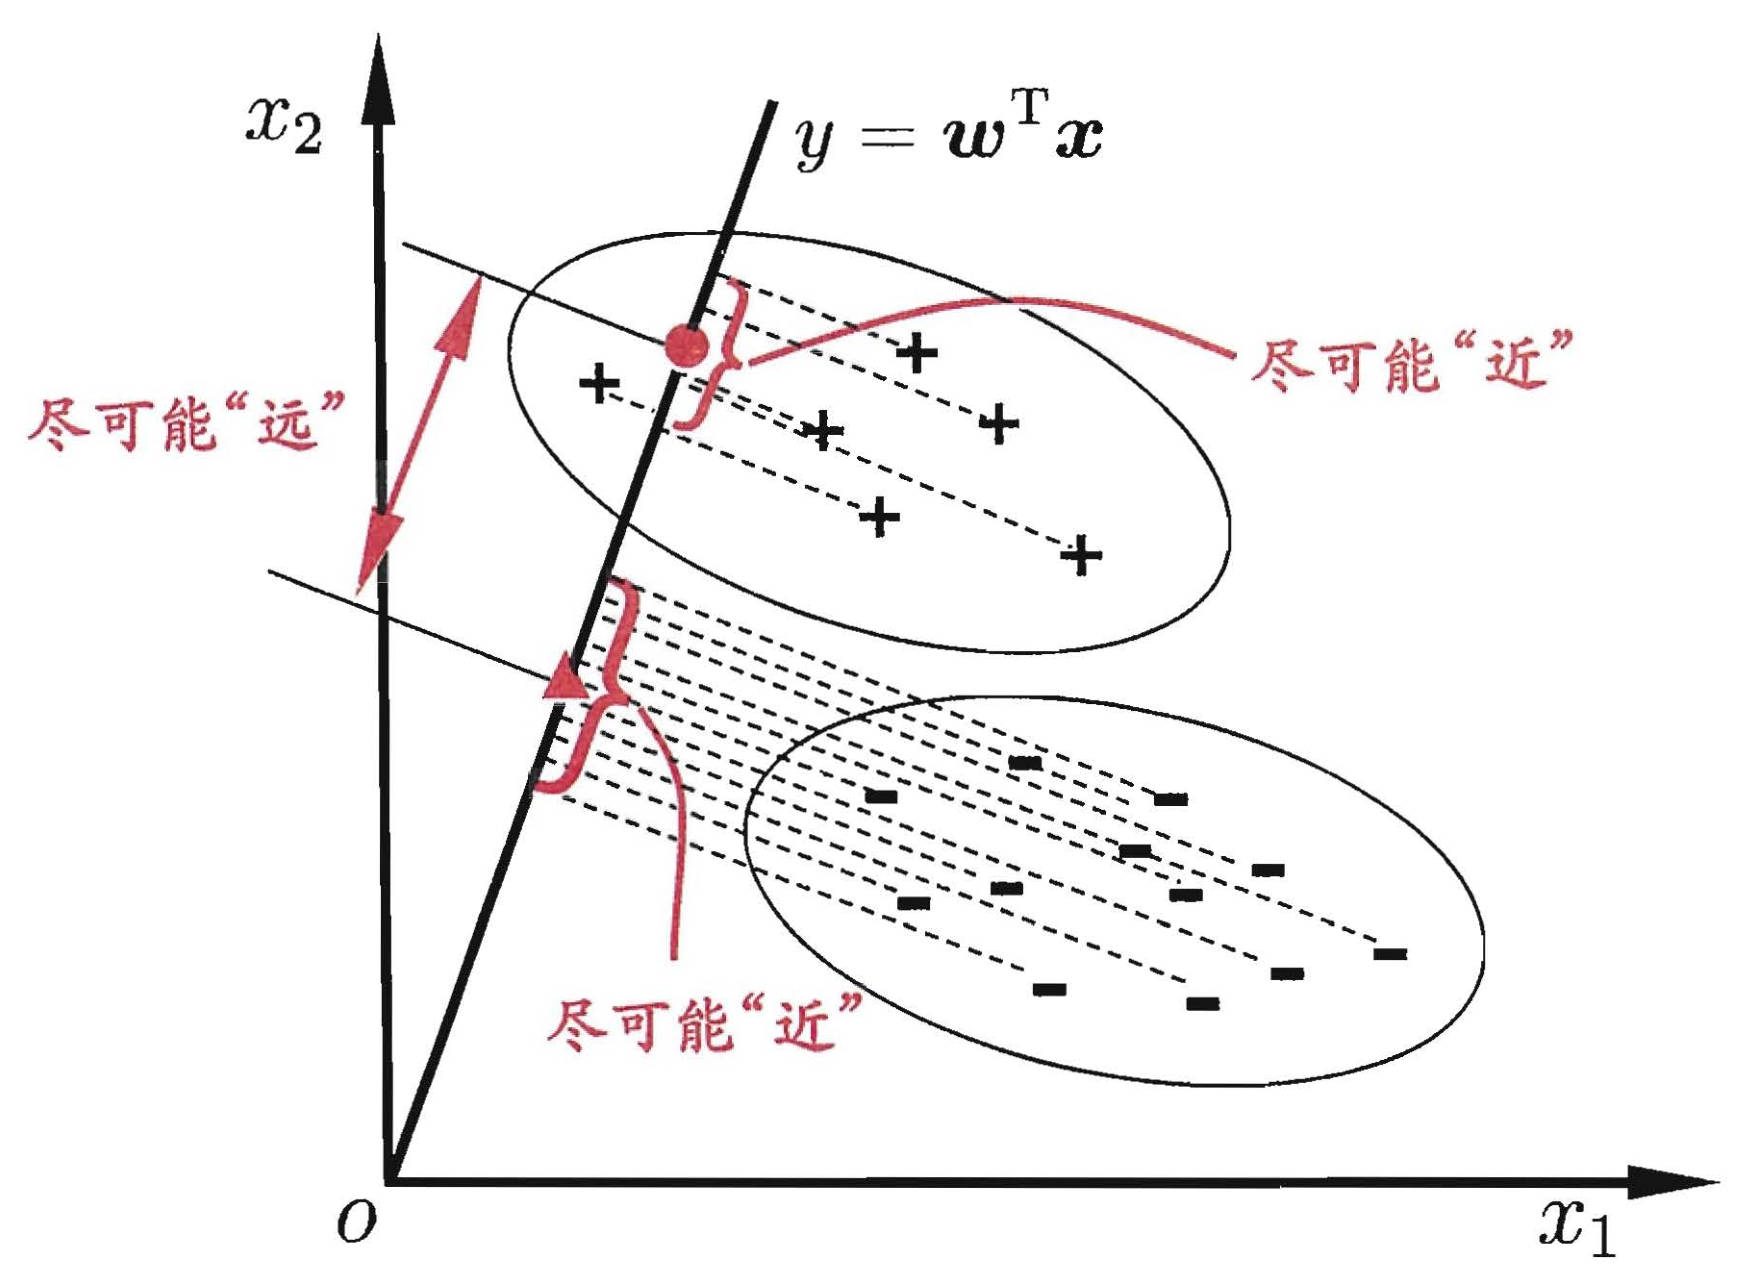
\includegraphics[width=0.5\linewidth]{textbook-fig3.3.jpg}
              \caption{教材图 3.3}
              \label{textbook_fig_3_3}
          \end{figure}
    \item[(2)] \textbf{[5pts]} 请参考题干中的介绍与 (1) 中的现象, 简要回答:
          \begin{itemize}
              \item [(a)] 对照题干中LDA的优化目的, PCA的优化目的是什么?
              \item [(b)] PCA相较于LDA有什么显著的不同点?
          \end{itemize}
    \item[(3)] \textbf{[5pts]} \textsf{下面, 我们先回顾教材第三章第四节中多分类 LDA 优化问题的矩阵形式. 考虑总类内散度是各个类别散度之和, 其矩阵形式为:
              $\Sw = \sum_{i=1}^{N} {\Sw}_i.$
              对于第 $i$ 个类别的类内散度矩阵定义如下:
              ${\Sw}_i = \sum_{\x \in X_i} (\x - \muBold_i) (\x - \muBold_i)^\transposed.$
              类似的, 总类间散度是各个类别中心相对于全局中心的散度之和, 其矩阵形式为:
              $\Sb = \sum_{i=1}^{N} {\Sb}_i.$
              对于第 $i$ 个类别的中心相对于全局中心的散度矩阵定义如下:
              ${\Sb}_i = m_i (\muBold_i - \muBold) (\muBold_i - \muBold)^\transposed.$}\\
          LDA事实上是在最小化\textbf{平均}类内散度和最大化\textbf{平均}类间散度, 其矩阵形式如 \eqref{lda-eigen} 所示. 其中, $d'$ 是降维后的维度, 严格小于数据维度 $d$.
          \begin{equation}
              \begin{aligned}
                  \max_{\W} \quad     & J(\W) = \frac{\tr{\W^\transposed \Sb \W}}{\tr{\W^\transposed \Sw \W}} = \frac{\tr{\W^\transposed \sbr{\sum_{i=1}^{N} {\Sb}_i} \W}}{\tr{\W^\transposed \sbr{\sum_{i=1}^{N} {\Sw}_i} \W}} = \frac{\frac{1}{N} \sum_{i=1}^{N} \tr{\W^\transposed {\Sb}_i \W}}{\frac{1}{N} \sum_{i=1}^{N} \tr{\W^\transposed {\Sw}_i \W}} \\
                  \mathrm{s.t.} \quad & \W^\transposed \W = \I_{d'}
              \end{aligned}
              \label{lda-eigen}
          \end{equation}

          \textbf{根据教材中的介绍, \eqref{lda-eigen} 可通过广义特征值分解进行求解.} 然而, 在某些现实场景下, 我们应用LDA的目的是提高分类准确率, 那么通常进一步希望\textbf{每个}类别散度尽可能小, \textbf{每个}类别中心相对于全局中心的散度尽可能大, \textbf{而非平均散度}. 因此, 考虑LDA的一种拓展形式:
          \begin{equation}
              \begin{aligned}
                  \max_{\W} \quad     & \sbr{\min_{i,j} J_{i,j}(\W)} = \frac{\min_{j} \{ \tr{\W^\transposed {\Sb}_j \W} \}}{\max_{i} \{ \tr{\W^\transposed {\Sw}_i \W} \}} \\
                  \mathrm{s.t.} \quad & \W^\transposed \W = \I_{d'}
              \end{aligned}
              \label{lda-pairwise}
          \end{equation}
          \textbf{请指出拓展形式 \eqref{lda-pairwise} 无法直接沿用原有形式 \eqref{lda-eigen} 的广义特征值求解算法的原因.} \\
          提示: 指出求解时存在变量间的循环依赖关系.
    \item[(4)] \textbf{[5pts]} \textsf{在线性代数中, 对于(半)正定矩阵 $\A, \B$, 若 $\sbr{\A-\B}$ 是正定矩阵, 则通常记作 $\A \succ \B$ 或 $\B \prec \A$; 若 $\sbr{\A-\B}$ 是半正定矩阵, 则通常记作 $\A \succcurlyeq \B$ 或 $\B \preccurlyeq \A$. 在优化问题中, 凸优化问题有多项式时间复杂度的理论保证, 能够高效求解. 凸优化问题的定义是: (i) 最小化的目标函数是凸函数, 或者最大化的目标函数是凹函数, 而且 (ii) 可行域是凸集. 可行域是所有满足约束条件的控制变量取值 (又称可行解) 构成的集合.} \\
          拓展形式 \eqref{lda-pairwise} 不能沿用原有形式 \eqref{lda-eigen} 的求解算法, 也不是凸优化问题. 为了高效求解, 需要探索一种将其转化成凸优化问题的方法. 已知原有形式 \eqref{lda-eigen} 可以松弛成如下凸优化问题:
          \begin{equation}
              \begin{aligned}
                  \max_{\W,r} \quad   & r                                             \\
                  \mathrm{s.t.} \quad & r \cdot \tr{\Sw \M} - \tr{\Sb \M} \leqslant 0 \\
                  \quad               & -r \leqslant 0                                \\
                  \quad               & \O \preccurlyeq \M \preccurlyeq \I_{d'}       \\
                  \quad               & \tr{\M} = d'                                  \\
              \end{aligned}
              \label{lda-slack}
          \end{equation}
          请仿照原有形式 \eqref{lda-eigen} 的松弛形式 \eqref{lda-slack}, 给出拓展形式 \eqref{lda-pairwise} 的松弛形式, 并证明拓展形式的松弛形式是凸优化问题, 即同时满足条件 (i) 和条件 (ii). \\
          \textcolor{red}{\textbf{本题表述存在问题, 形如 $x \cdot y - z \leqslant 0$ 或者 $x \cdot y - z = 0$ 的约束不构成凸集合, 正确的表述应为证明 (4.3) 除 $r \cdot \tr{\Sw \M} - \tr{\Sb \M} \leqslant 0$ 以外构成凸优化问题.}}
    \item[(5)] \textbf{[5pts]} (\textsf{本题为附加题, 得分计入卷面分数, 但本次作业总得分不超过 100 分}) 请证明:
          \begin{itemize}
              \item [(a)] 松弛形式 \eqref{lda-eigen} 和原有形式 \eqref{lda-slack} 的约束条件不等价;
              \item [(b)] 当 $r \cdot \tr{\Sw \M} - \tr{\Sb \M} = 0$ 时, \eqref{lda-slack} 的可行域是 \eqref{lda-eigen} 可行域的凸包 (Convex Hull). 即: \eqref{lda-slack} 的可行解可以表示成 \eqref{lda-eigen} 的可行解的线性组合.
          \end{itemize}
          进而, \eqref{lda-slack} 的可行域是包含 \eqref{lda-eigen} 的可行域的最小凸集, 即 \eqref{lda-slack} 对 \eqref{lda-eigen} 的放松程度是最小的, 因而能够使得凸问题 \eqref{lda-slack} 的解尽可能的接近原问题 \eqref{lda-eigen} 的解.
\end{enumerate}

\begin{solution}
    此处用于写解答 (中英文均可)
    \begin{itemize}
        \item[(1)] 大致如下图~\ref{textbook_fig_3_3_pca}.
              \begin{figure}[htbp]
                  \centering
                  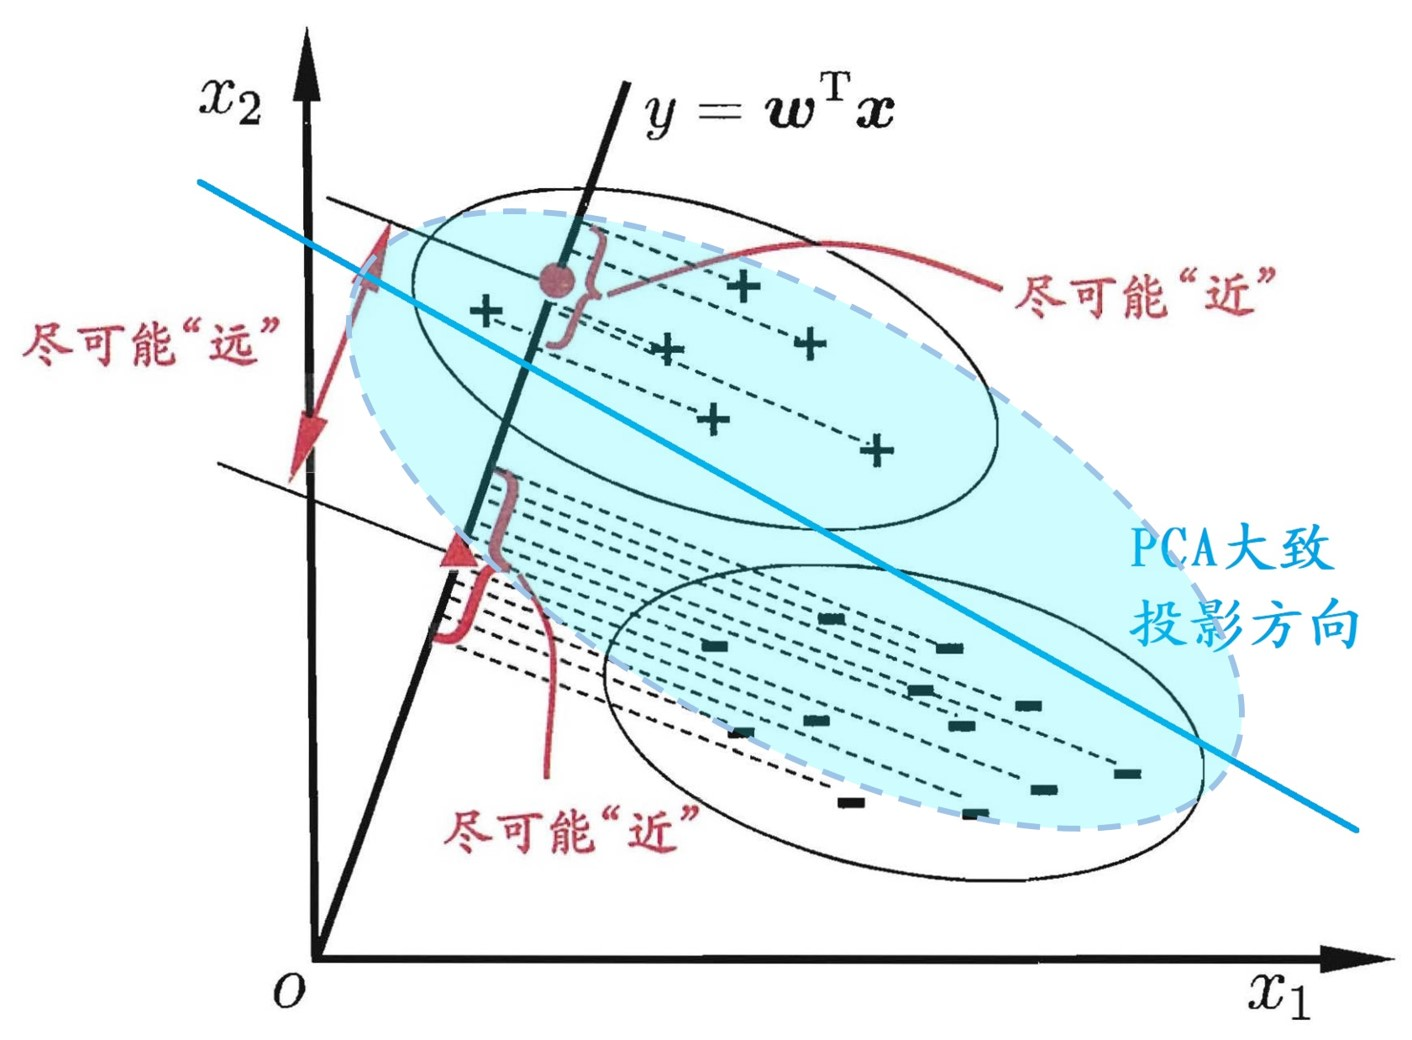
\includegraphics[width=0.5\linewidth]{textbook-fig3.3-pca.jpg}
                  \caption{教材图 3.3, PCA的大致投影方向}
                  \label{textbook_fig_3_3_pca}
              \end{figure}
        \item[(2)] PCA 不包含标签信息, 最大化类别无关的全局散度.
        \item[(3)] 求解 $\W$ 依赖于 $i,j$, 求解 $i,j$ 依赖于 $\W$.
        \item[(4)] 省略约束条件 $- r \leqslant 0$, $\O \preccurlyeq \M \preccurlyeq \I_{d}$, $\tr{\M} = d'$, 如下三种形式均可.
              证明要点: \textbf{半正定锥 (Positive Semi-definite Cone) 凸}; 凸函数小于等于一定值的解集凸; $\tr{\cdot}$, $\max$, $-\min$ 和线性运算保凸.
              $$
                  \begin{aligned}
                      \max_{\M,r,a,b} \quad     & r                                                                                         \\
                      \operatorname{s.t.} \quad & r \cdot \max_i \tr{{\Sw}_i \M} - \min_j \tr{{\Sb}_j \M} \leqslant 0                       \\
                      \operatorname{s.t.} \quad & r \cdot \tr{{\Sw}_i \M} - \tr{{\Sb}_j \M} \leqslant 0               & \forall i,j \in [N] \\
                      \operatorname{s.t.} \quad & r \cdot a - b \leqslant 0                                                                 \\
                      \quad                     & \tr{{\Sw}_i \M} - a \leqslant 0                                     & \forall i \in [N]   \\
                      \quad                     & b - \tr{{\Sb}_j \M} \leqslant 0                                     & \forall j \in [N]   \\
                  \end{aligned}
              $$
        \item[(5-a)] $\tr{\A\B\C} = \tr{\B\C\A} = \tr{\C\B\A}$; $\M = \W\W^\transposed$, $\M$ 无法表达正交性约束.
        \item[(5-b)] 注意 $\{\M\}$ 和 $\{\W\W^T\}$ 的正交相似变换不变性. 幂集记作 $\mathcal{P}$, 考虑集合函数
              $$\sigma: \mathcal{P}(\Real^{d}) \to \mathcal{P}(\Real^{d \times d}), \qquad \sigma(\{\lambdaBold\}) = \{\Q^{-1} \operatorname{diag}(\lambdaBold) \Q \mid \Q^\transposed \Q = \I\}.$$
              注意到 $\M = \sum_{i=1}^{d} \lambda_i \v_i \v_i^\transposed$, $\W\W^\transposed = \sum_{i=1}^{d'} \v_i \v_i^\transposed$. 因此 $\{\M\}$ 由 $\{\lambdaBold \mid \bm{0} \preccurlyeq \lambdaBold \preccurlyeq \bm{1}, \bm{1}^\transposed \lambdaBold = d'\}$ 生成, $\{\W\W^\transposed\}$ 由 $\{\lambdaBold \mid \forall i \in \{1, \cdots, d\}, \lambdaBold_i \in \{0, 1\}, \bm{1}^\transposed \lambdaBold = d'\}$ ($d$ 维 ``$d'$-hot'' 向量) 生成. \\
              不难发现 $\sigma^{-1}(\{\M\})$ 是一个闭合多面体/凸集 (Polygon / Convex Set), 而 $\sigma^{-1}(\{\W\W^\transposed\})$ 恰好构成其顶点/极点 (Vertex / Extreme Point), 注意到 $\sigma$ 具有保凸性, 从而凸包得证. \\
              \textsf{注1: 在正交相似变换 (Orthogonal Similar Transformation), $\tilde{\M} = \Q^{-1} \M \Q$, $\Q^\transposed \Q = \I$.} \\
              \textsf{注2: 极点是不能用凸集内其他点组合表示的点, 凸集中所有点可表示成极点的组合.} \\
              \textsf{注3: 初等证明等价于 $d$ 维 ``$d'$-hot'' 向量对应的 Toeplitz Matrix 的非奇异性, 非常困难.} \\
    \end{itemize}
\end{solution}


\newpage

\section{[25pts] 编程实验: LDA 与多分类}

\begin{tcolorbox}
    \textbf{[注意事项]} 请不要修改或提交 \texttt{utils.py}; 在合理范围内, 运行时间和错误率不作为评分依据. 实现过程中只允许使用 NumPy 和 SciPy 提供的矩阵运算接口, 否则相应题目不计入分数.

    此外, 对于题 (3,4,5), 如果调用 Sci-Kit Learn 实现二分类模型, 基于二分类模型实现多分类模型, 并且画出相应图像, 可计入题 (4,5) 得分, 但不计入题 (3) 得分.

    \textbf{[符号约定]} \texttt{x} 是形状为 \texttt{(m, d)} 的矩阵, 其元素为32位浮点数; 在题 (1,3,4,5) 中, \texttt{y} 是形状为 \texttt{(m,)} 的向量, 其元素为32位整数; 在题 (2) 中, \texttt{y} 是形状为 \texttt{(m, 2)} 的向量, 其元素为32位浮点数. 其中: \texttt{m} 为样例个数, \texttt{d} 为样例维度; 标签从 \texttt{0} 开始, 例如共20类时, 标签依次是 $\{\mathtt{0}, \cdots, \mathtt{19}\}$.
\end{tcolorbox}

\begin{enumerate}
    \item[(1)] \textbf{[5pts]} 根据 \texttt{main.py} 中的框架代码, 实现LDA降维, 通过 \texttt{lda\_sanity\_check} 测试, 并在 \texttt{HW2.pdf} 中展示运行后的终端输出截图.
    \item[(2)] \textbf{[5pts]} 基于 (1) 分别把训练数据和测试数据降至两维, 并绘制在同一张散点图上, 在 \texttt{HW2.pdf} 中展示. 注意: 同类别的点应当使用同一颜色, 不同类别的数据点应当使用不同颜色.
    \item[(3)] \textbf{[5pts]} 分类任务可以被归结为一种特殊的回归任务, 可参考 \texttt{sklearn} 中的内容: \href{https://scikit-learn.org/stable/modules/linear_model.html#classification}{[Link]}. 对于二分类任务, 我们任选一类作为正类, 另一类成为负类. 对于正类样本 $\x_+$, 约定 $y_+ = 1$, 对于负类样本 $\x_-$, 约定 $y_- = -1$, 对于训练得到的分类器 $f$ 和测试样例 $\x$, 如果 $f(\x) \geqslant 0$ 预测为正类, 否则预测为负类. \\根据框架代码, 按照上述约定实现基于岭回归的二分类模型, 通过\\ \texttt{classifier\_2\_sanity\_check} 测试, 并在 \texttt{HW2.pdf} 中展示运行后的终端输出截图.
    \item[(4)] \textbf{[5pts]} 基于 (3) 中的二分类模型, 通过 OvR 策略将其拓展为多分类模型, 通过\\ \texttt{classifier\_n\_sanity\_check} 测试, 最后在 \texttt{HW2.pdf} 中展示运行后的终端输出截图.\\提示: 判断测试样例的预测结果时, 可以依照教材实现, 即若有多个分类器预测为正类或者没有分类器预测为正类, 则考虑各分类器的预测置信度 ($f(\x)$ 之值), 选择置信度最大的类别标记作为分类结果.
    \item[(5)] \textbf{[5pts]} 基于 (4) 绘制并在 \texttt{HW2.pdf} 中展示\textbf{训练错误率和测试错误率随 $\lambda$ 变化的折线图}. 注意: 图像横轴为 $\lambda$; 训练错误率和测试错误率应当使用不同颜色的曲线.
\end{enumerate}

\begin{solution}
    此处用于写解答 (中英文均可)
    \begin{enumerate}
        \item[(1,3)] NumPy 代码与矩阵运算一一对应.
        \item[(2)] 特点: 训练数据完全可分, 泛化能力很差.
        \item[(4)] \texttt{RidgeN} 递归调用 \texttt{Ridge2}.
        \item[(5)] 特点: 训练数据误差为零, 泛化能力随正则化力度增大而增强.
              \begin{figure}
                  \centering
                  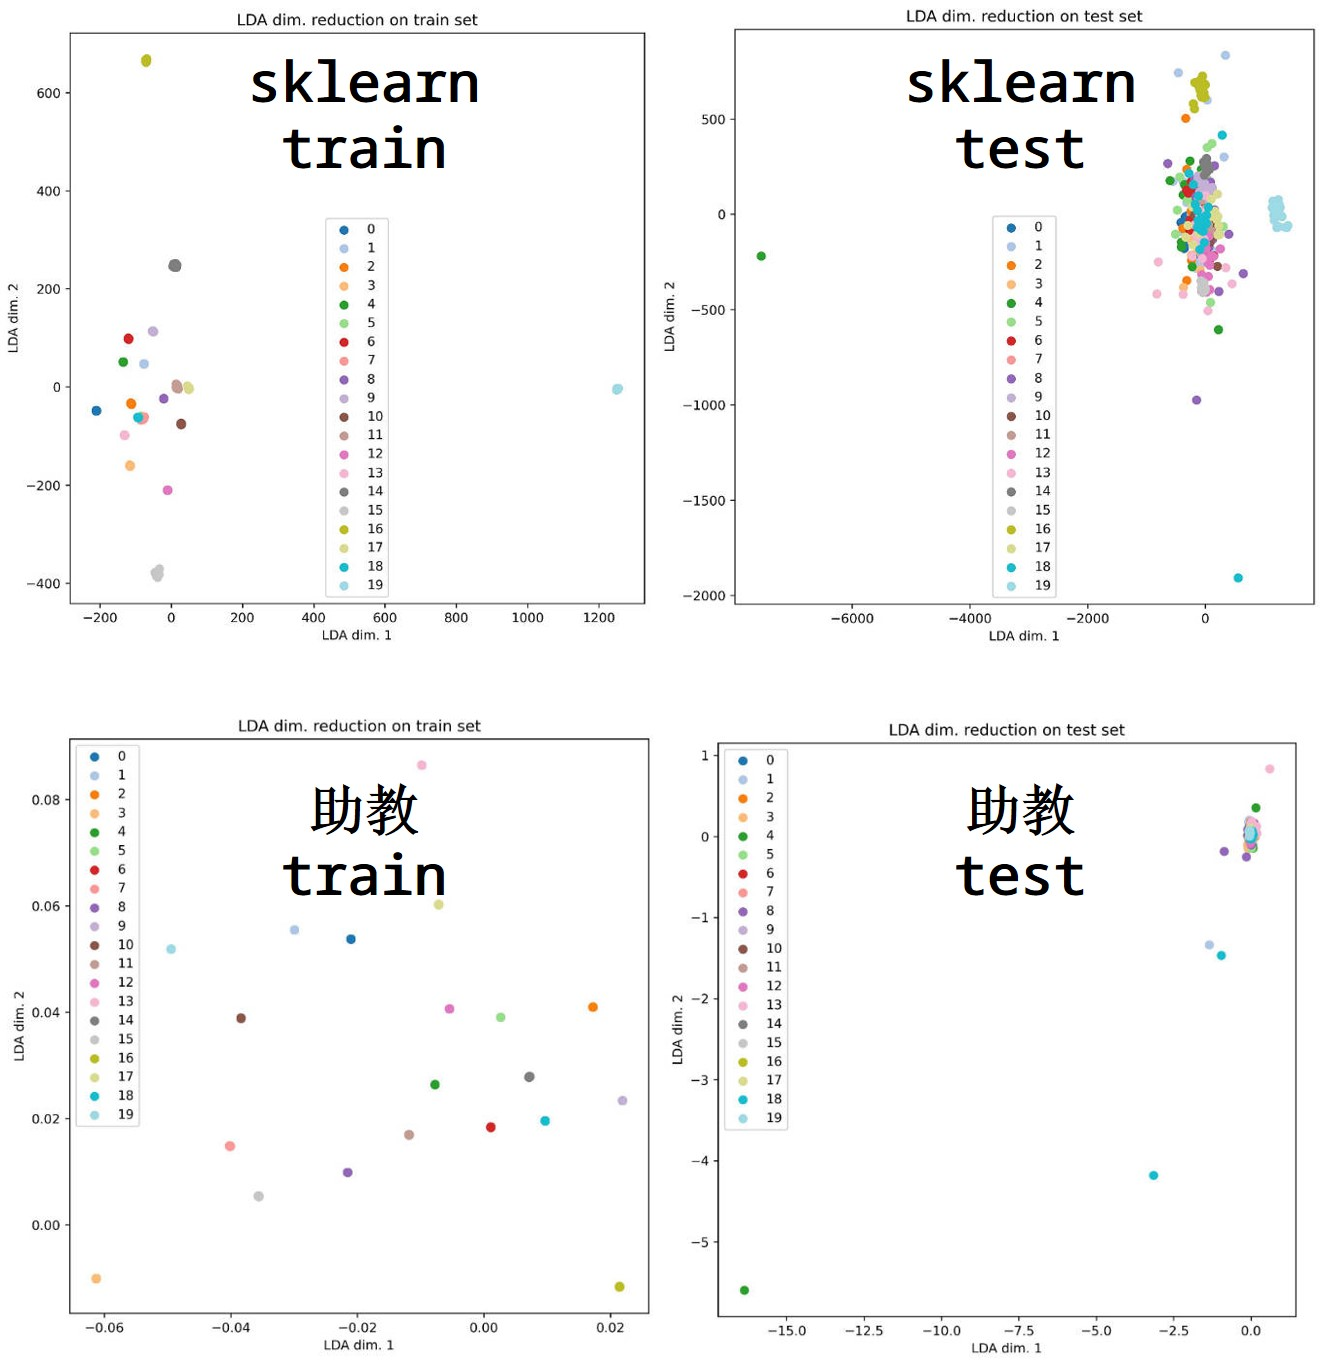
\includegraphics[width=0.8\textwidth]{./programming-lda.jpg}
                  \caption{\texttt{LDA}}
              \end{figure}
              \begin{figure}
                  \centering
                  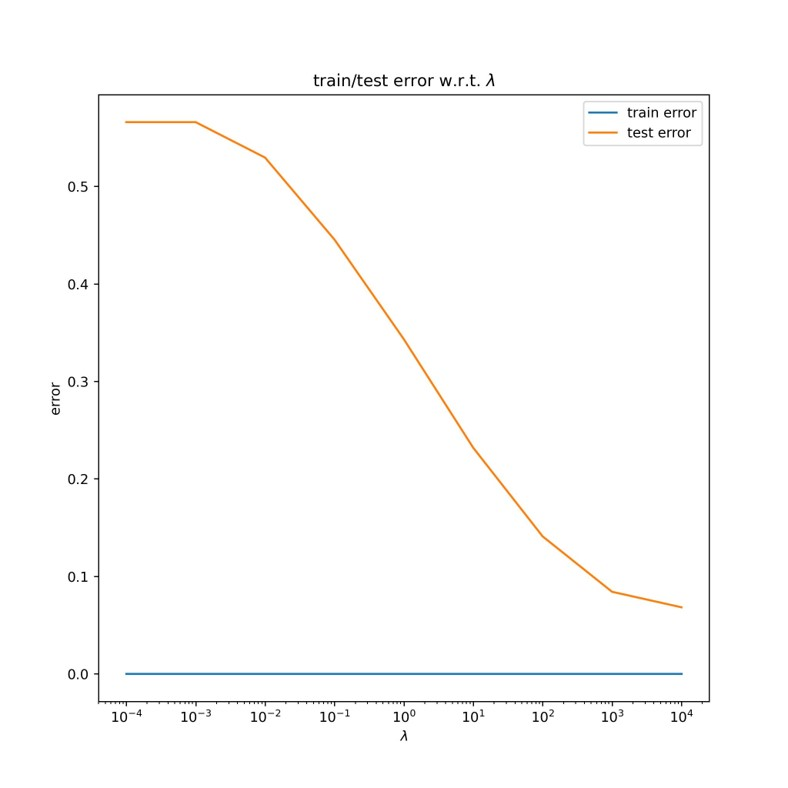
\includegraphics[width=0.4\textwidth]{./programming-ridge.jpg}
                  \caption{\texttt{RidgeN}}
              \end{figure}
    \end{enumerate}
\end{solution}

\newpage

% \section*{Acknowledgments}
% 允许与其他同样未完成作业的同学讨论作业的内容, 但需在此注明并加以致谢; 如在作业过程中, 参考了互联网上的资料或大语言模型的生成结果, 且对完成作业有帮助的, 亦需注明并致谢.

\end{document}
